  \documentclass[final]{beamer} % beamer 3.10: do NOT use option hyperref={pdfpagelabels=false} !
  %\documentclass[final,hyperref={pdfpagelabels=false}]{beamer} % beamer 3.07: get rid of beamer warnings
  \mode<presentation> {  %% check http://www-i6.informatik.rwth-aachen.de/~dreuw/latexbeamerposter.php for examples
    \usetheme{Berlin}    %% you should define your own theme e.g. for big headlines using your own logos 
    % \usetheme{Warsaw}
    % \usetheme{Montpellier}
    % \usetheme{Singapore}
    % \usetheme{crane}
    % \usetheme{Aachen}
    % \usetheme{Oldi6}
    % \usetheme{I6td}
    % \usetheme{I6dv}
    % \usetheme{I6pd}
    % \usetheme{I6pd2}
  }
  \usepackage{tikz}

  \usebackgroundtemplate{%
  \tikz\node[opacity=0.50] {\hskip-2ex \includegraphics[trim = 300mm 0mm 0mm -80mm,clip,height=\paperheight,keepaspectratio=true]{./FIGS/Paralithodes_camtschaticus}};}

  \addtobeamertemplate{block begin}{\pgfsetfillopacity{0.5}}{\pgfsetfillopacity{1}}
  \addtobeamertemplate{block alerted begin}{\pgfsetfillopacity{0.5}}{\pgfsetfillopacity{1}}
  \addtobeamertemplate{block example begin}{\pgfsetfillopacity{0.5}}{\pgfsetfillopacity{1}}



  \setbeamerfont{itemize}{size=\normalsize}
  \setbeamerfont{itemize/enumerate body}{size=\normalsize}
  \setbeamerfont{itemize/enumerate subbody}{size=\normalsize}

  \setbeamertemplate{caption}[numbered]

  % additional packages
  \usepackage{times}
  \usepackage{amsmath,amsthm, amssymb, latexsym, bm}
  \usepackage{exscale}
  \usepackage{ragged2e}
  %\boldmath
  \usepackage{booktabs, array}
  %\usepackage{rotating} %sideways environment
  \usepackage[english]{babel}
  \usepackage[latin1]{inputenc}
  \usepackage[orientation=landscape,size=custom,width=200,height=200,scale=1.95]{beamerposter}
  \listfiles
  \graphicspath{{figures/}}
  \graphicspath{{FIGS/}}
  % Display a grid to help align images
  %\beamertemplategridbackground[1cm]

  \title[\url{https://github.com/seacode/gmacs}]{GMACS: A Generalized Size-Structured Model and Stock Reduction Analysis}
  \author[Martell et al.]{Steve Martell, James Ianelli, and Dave Fournier}
  \institute[IPHC]{International Pacific Halibut Commission, Alaska Fisheries Science Center, and Otter Research}
  \date[Photo Credit: S. Isachenko]{May 2015}

  % abbreviations
  \usepackage{xspace}
  \makeatletter
  \DeclareRobustCommand\onedot{\futurelet\@let@token\@onedot}
  \def\@onedot{\ifx\@let@token.\else.\null\fi\xspace}
  \def\eg{{e.g}\onedot} \def\Eg{{E.g}\onedot}
  \def\ie{{i.e}\onedot} \def\Ie{{I.e}\onedot}
  \def\cf{{c.f}\onedot} \def\Cf{{C.f}\onedot}
  \def\etc{{etc}\onedot}
  \def\vs{{vs}\onedot}
  \def\wrt{w.r.t\onedot}
  \def\dof{d.o.f\onedot}
  \def\etal{{et al}\onedot}
  \makeatother

  \newcommand{\fspr}{F$_{\rm{SPR=35\%}}$}
  \newcommand{\bspr}{B$_{\rm{SPR=35\%}}$}
  \newcommand{\rspr}{R$_{\rm{SPR=35\%}}$}
  \newcommand{\fofl}{F$_{\rm{OFL}}$}

  \usepackage{pifont}% http://ctan.org/pkg/pifont
  \newcommand{\cmark}{\ding{51}}%
  \newcommand{\xmark}{\ding{55}}%


  \definecolor{cM1}{rgb}{0.9608,0.4706,0.4392}
  \definecolor{cM2}{rgb}{0.4902,0.6745,0.1216}
  \definecolor{cM3}{rgb}{0.2275,0.7765,0.7922}
  \definecolor{cM4}{rgb}{0.7765,0.5020,0.9843}

\setbeamertemplate{headline}{
 \leavevmode
  \begin{columns}
   \begin{column}{.1\linewidth}
   \end{column}
   \begin{column}{.8\linewidth}
    \vskip1cm
    \centering
    \usebeamercolor{title in headline}{\color{blue}\Huge{\textbf{\inserttitle}}\\[0.5ex]}
    \usebeamercolor{author in headline}{\color{fg}\Large{\insertauthor}\\[1ex]}
    \usebeamercolor{institute in headline}{\color{fg}\large{\insertinstitute}\\[1ex]}
    \vskip1cm
   \end{column}
   \begin{column}{.1\linewidth}
    
\includegraphics{./FIGS/QRCode.png}
   \end{column}
   \vspace{1cm}
  \end{columns}
 \vspace{0.5in}
 \hspace{0.5in}\begin{beamercolorbox}[wd=48in,colsep=0.15cm]{cboxb}\end{beamercolorbox}
 \vspace{0.1in}
}

\setbeamertemplate{footline}
{
  \leavevmode%
  \hbox{%
    \pgfsetfillopacity{0}\begin{beamercolorbox}[wd=.333333\paperwidth,ht=2.25ex,dp=4ex,center]{author in head/foot}%
      \usebeamerfont{author in head/foot}\pgfsetfillopacity{1}\color{fg}\Large\insertshortauthor~~(\insertshortinstitute)
    \end{beamercolorbox}%
    \pgfsetfillopacity{0}\begin{beamercolorbox}[wd=.333333\paperwidth,ht=2.25ex,dp=4ex,center]{title in head/foot}%
      \usebeamerfont{title in head/foot}\pgfsetfillopacity{1}]\Large\insertshorttitle
    \end{beamercolorbox}%
    \pgfsetfillopacity{0}\begin{beamercolorbox}[wd=.333333\paperwidth,ht=2.25ex,dp=4ex,right]{date in head/foot}%
      \usebeamerfont{date in head/foot}\pgfsetfillopacity{1}\Large\insertshortdate{}\hspace*{2em}
      % \insertframenumber{} / \inserttotalframenumber\hspace*{2ex}
    \end{beamercolorbox}}%
  \vskip0pt%
}


%%%%%%%%%%%%%%%%%%%%%%%%%%%%%%%%%%%%%%%%%%%%%%%%%%%%%%%%%%%%%%%%%%%%%%%%%%%%%%%%%%%%%%%%%%%%%%%%%%%%%%%%%%%%
%%%%%%%%%%%%%%%%%%%%%%%%%%%%%%%%%%%%%%%%%%%%%%%%%%%%%%%%%%%%%%%%%%%%%%%%%%%%%%%%%%%%%%%%%%%%%%%%%%%%%%%%%%%%









  % \usepackage[english]{babel}
  % \usepackage[latin1]{inputenc}
  % \usepackage{amsmath,amsthm, amssymb, latexsym}
  % %\usepackage{times}\usefonttheme{professionalfonts}  % times is obsolete
  % \usefonttheme[onlymath]{serif}
  % \boldmath
  % % \usepackage[orientation=landscape,size=a0,scale=1.4,debug]{beamerposter}                       % e.g. for DIN-A0 poster
  % %\usepackage[orientation=portrait,size=a1,scale=1.4,grid,debug]{beamerposter}                  % e.g. for DIN-A1 poster, with optional grid and debug output
  % \usepackage[size=custom,width=200,height=200,scale=2,debug]{beamerposter}                     % e.g. for custom size poster
  % %\usepackage[orientation=portrait,size=a0,scale=1.0,printer=rwth-glossy-uv.df]{beamerposter}   % e.g. for DIN-A0 poster with rwth-glossy-uv printer check
  % % ...
  % %
  % \title[Fancy Posters]{Making Really Fancy Posters with \LaTeX}
  % \author[Dreuw \& Deselaers]{Philippe Dreuw and Thomas Deselaers}
  % \institute[RWTH Aachen University]{Human Language Technology and Pattern Recognition,RWTH Aachen University}
  % \date{Jul. 31th, 2007}
  \begin{document}
  \begin{frame}{} 
    % \maketitle
    % \vfill
    \begin{columns}[t]
      
      %% ------------------------------------------------------------------------------ %%
      %% COLUMN 1
      \begin{column}{.3\linewidth}
        \vspace{3in}
        %%%%%%%%%%%%%%%%%%%%%%%%%%%%%%%%%%%%%%%%%%%%%%%%%%%%%%%%%%%%%%%%%%%%%%%%%%%%%%%
        \begin{block}{\large Data Inputs}
          \begin{table}
          \centering
          %\footnotesize
          \caption{Required and optional input data for GMACS.}
          \begin{tabular}{@{} p{.7\linewidth} c r @{}}
            \toprule
            % Features                                                             & Dim.            & [\%WER] \\
            Data Type                                  & Symbol  & Required \\
            \midrule
            History of catch removals                  &  $C_t$  & yes      \\
            History of discards                        &  $D_t$  & no       \\
            \addlinespace
            \addlinespace
            Relative abundance data (\eg, CPUE)        &  $I_t$  & no       \\
            \addlinespace
            \addlinespace
            Size composition (sex,type,shell,maturity) &$\bm{Q}_{h,p,o,m}$ & no       \\
            Growth increment data                      &  $g_h$    & no       \\
            Size Transition Matrix                     &$\bm{G}_{h}$ & no       \\
            \bottomrule
          \end{tabular}
          \label{tab:data_inputs}
          \end{table}
        \end{block}
        %%%%%%%%%%%%%%%%%%%%%%%%%%%%%%%%%%%%%%%%%%%%%%%%%%%%%%%%%%%%%%%%%%%%%%%%%%%%%%%
        \vskip1ex
        %%%%%%%%%%%%%%%%%%%%%%%%%%%%%%%%%%%%%%%%%%%%%%%%%%%%%%%%%%%%%%%%%%%%%%%%%%%%%%%
        \begin{block}{\large General Size-structured Equilibrium Model}


          Given a vector $\bm{n} = (n_1,n_2,\ldots,n_m)$ that represents the number of individuals in discrete
          size bins in a given year.  Each year the numbers in each size bin are subject to 
          growth and survival $\bm{A}$ and the addition of recruits $\bm{r}$.
          Assuming growth and survival is a linear function of the number of 
          individuals in each size bin, then the following matrix equation represents
          the steady-state or equilibrium conditions:
          \[\bm{n} = \bm{A}\bm{n} + \bm{r}\]
          with the equilibrium solution for the numbers-at-size given by
          \[\bm{n} = -(\bm{A} - \bm{I})^{-1} (\bm{r})\]
          where $\bm{I}$ is the $m$ x $m$ identity matrtix. In practical terms, the 
          challenge is in developing the matrix $\bm{A}$ and the vector of new recruitment
          $\bm{r}$.\\[1ex]

          Our approach accomodates the dynamics of molting probabilities, and 
          jointly modeling the abundance of new and old shell crabs and maturity state.
        \end{block}
        %%%%%%%%%%%%%%%%%%%%%%%%%%%%%%%%%%%%%%%%%%%%%%%%%%%%%%%%%%%%%%%%%%%%%%%%%%%%%%%
        \vskip1ex
        %%%%%%%%%%%%%%%%%%%%%%%%%%%%%%%%%%%%%%%%%%%%%%%%%%%%%%%%%%%%%%%%%%%%%%%%%%%%%%%

        \begin{block}{\large Generalized Model Notation (equilibrium conditions)}
          \begin{table}
            \centering
            % \caption{Mathematical equations and notation for a steady-state length based model.}
            \label{tab:equilibrium_model}
            \vskip-2ex
            % \tableEq
              \begin{align}
                % \hline \nonumber \\
                &\mbox{\underline{model parameters}} \nonumber\\
                &\Theta = (M,\alpha_r,\beta_r,R_0,\kappa) \label{T1.1}\\[1ex]
                &M > 0 , \alpha_r > 0, \beta_r > 0, R_0>0,\kappa > 1.0, \quad \mbox{constraints}\label{T1.2}\\[1ex]
                &\Phi = (\alpha,\beta,\varphi), \quad \mbox{Size-transition parameters} \label{T1.3}\\[2ex]
                %%
                %%
                &\mbox{\underline{size-transition matrix $\bm{G}$}} \nonumber \\
                %vector of length intervals
                &\vec{l},\vec{x} \quad \mbox{vector of size intervals and midpoints, respectively} \nonumber\\[1ex]
                % Growth increment
                &a_{l} = (\alpha + \beta l)/\varphi \label{T1.4} \\[1ex]
                %Size transition matrix
                &p({l},{l'}) =\pmb{G}= \int_{l}^{l+\Delta l}
                    \frac{ l^{(a_{l}-1)} \exp(l/\varphi) }
                    { \Gamma(a_{l}) l^{(a_{l})} } dl \label{T1.5} \\[2ex]
                %%
                %%
                &\mbox{\underline{recruitment size-distribution}} \nonumber \\
                & \alpha = \alpha_r / \beta_r  \\[1ex]
                % Size distribution of new recruits
                &p[\bm{r}] = \int_{x_l-0.5\Delta x}^{x_l+0.5\Delta x}
                  \frac{x^{(\alpha-1)}\exp(- x / \beta_r)}{\Gamma(\alpha)\beta_r^\alpha}dx
                    \label{T1.7}\\[1ex]
                &\pmb{r} = 0.5 p[\bm{r}] \ddot{R} \label{T1.8}\\[2ex]
                %%
                %%
                &\mbox{\underline{growth and survival}} \nonumber \\
                % &\pmb{U} = \exp(-M) (\pmb{I}_n)_{l,l'} \label{T1.9} \\
                %unfished
                &\pmb{A} = \pmb{G} [\exp(-M) (\pmb{I}_n)_{l,l'}] \quad \mbox{unfished}\label{T1.10}\\[1ex]
                % &\pmb{F} = \exp(-M - \pmb{f}_{h,l}) (\pmb{I}_n)_{l,l'} \label{T1.11}\\
                %fished
                &\pmb{B} = \pmb{G} [\exp(-M - \pmb{f}_{l}) (\pmb{I}_n)_{l,l'}] \quad \mbox{fished} \label{T1.12}\\[2ex]
                %%
                %%
                &\mbox{\underline{survivorship to size-interval}} \nonumber \\
                & \bm{u}   = -(\bm{A} - (\bm{I}_n)_{l,l'})^{-1} (p[\bm{r}]) \quad \mbox{unfished} \label{T1.13a}\\[1ex]
                & \bm{v}   = -(\bm{B} - (\bm{I}_n)_{l,l'})^{-1} (p[\bm{r}]) \quad \mbox{fished}   \label{T1.13b}\\[2ex]
                %%
                %%
                &\mbox{\underline{steady-state conditions}}\nonumber \\
                % & \pmb{v} = -(\pmb{A}-(\pmb{I}_n)_{l,l'})^{-1} (\pmb{r})\label{T1.13}\\
                & B_0 = R_0 \phi_B, \quad\mbox{where} \quad \phi_B=  \sum_l \pmb{u}_{l} w_{l} m_{l} \label{T1.14}\\[1ex]
                % & \pmb{n} = -(\pmb{B}-(\pmb{I}_n)_{l,l'})^{-1} (\pmb{r})\label{T1.15}\\
                & \tilde{B} = \tilde{R} \tilde{\phi}_B \quad\mbox{where}\quad \tilde{\phi}_B= \quad \sum_l \pmb{v}_{l} w_{l} m_{l} \label{T1.16}\\[2ex]
                %%
                %%
                &\mbox{\underline{stock-recruitment parameters}}\nonumber\\
                &s_o = \kappa R_0 / B_0 \label{T1.17}\\[1ex]
                &\beta = (\kappa -1)/B_0 \label{T1.18}\\[1ex]
                &\tilde{R} = \frac{s_o \tilde{\phi}_B -1}{\beta \tilde{\phi}_B} \label{T1.19}
                %%
                %%
                % \hline \hline \nonumber
              \end{align}
            % \normalEq
            \end{table}
            % \vskip-2ex
        \end{block}
        %%%%%%%%%%%%%%%%%%%%%%%%%%%%%%%%%%%%%%%%%%%%%%%%%%%%%%%%%%%%%%%%%%%%%%%%%%%%%%%

      \end{column}
      %% ------------------------------------------------------------------------------ %%







      %% ------------------------------------------------------------------------------ %%
      %% COLUMN 2
      \begin{column}{.3\linewidth}
        \vspace{-2in}
        %%%%%%%%%%%%%%%%%%%%%%%%%%%%%%%%%%%%%%%%%%%%%%%%%%%%%%%%%%%%%%%%%%%%%%%%%%%%%%%
        \begin{block}{\centering \large \textbf{Abstract}}
          \justifying
          Stock reduction analysis (SRA) is a data-poor technique that typically just uses historical 
          catch information to estimate recruitment rates needed to explain those historical catches.  
          The method is easily extended to accommodate sparse information on trends in abundance, 
          composition information, and tagging data.  Estimation of model parameters using maximum 
          likelihood or Bayesian methods is possible.  GMACS is a generalized framework for size-structured 
          models suitable for data-poor to data-rich assessments.  Reference points are derived from 
          steady-state conditions by solving matrix equations that represent size-dependent mortality 
          and growth.   Our results show how the scalability of GMACS can be used as an integrated
          data-poor assessment method. Next steps include the evaluation of such ``simple`` methods testing 
          simulated data generated from within GMACS (or from a separate R package) but configured to have 
          greater complexity of underlying dynamics (e.g., time-varying natural mortality))
        \end{block}
        \vspace{2in}
        %%%%%%%%%%%%%%%%%%%%%%%%%%%%%%%%%%%%%%%%%%%%%%%%%%%%%%%%%%%%%%%%%%%%%%%%%%%%%%%
        \vskip1ex
        %%%%%%%%%%%%%%%%%%%%%%%%%%%%%%%%%%%%%%%%%%%%%%%%%%%%%%%%%%%%%%%%%%%%%%%%%%%%%%%
        \begin{block}{\large Size-based selectivity, retention, and fishing mortality}
          \begin{table}
            \centering
            % \caption{Size-based selectivity, retention and fishing mortality.}
            \label{tab:fishing_mortality}
            % \tableEq
            \vskip-2ex
            \begin{align}
            % \hline \nonumber
            &\mbox{\underline{Parameters}}& \nonumber \\
            & \ln(f), a,\sigma_{s},\lambda,\sigma_{y},\xi \label{T4.1} & \xi=\mbox{Discard mortality} \\[1ex]
            % & \sum_i \bm\Psi_{k,i} = 0 \label{T4.2}\\[2ex]
            %%
            %%
            &\mbox{\underline{Selectivity \& retention}} &\nonumber \\
            &s_{l} = (1 + \exp(-(l-a )/ \sigma_{s}))^{-1}\label{T4.3} & \mbox{Capture probability}\\[1ex]
            &y_{l} = (1 + \exp(-(\lambda - l) / \sigma_{y}))^{-1}&\mbox{Retention probability}\label{T4.4}\\[1ex]
            &\nu_{l}  = s_{l} [y_{l} + (1-y_{l})\xi]&\mbox{Joint probability of dying from fishing}\label{T4.5}\\[2ex]
            %%
            %%
            &\mbox{\underline{Fishing mortality}}& \nonumber \\
            & F = \exp(\ln(f) ) &\mbox{Instantaneous fishing mortality}\label{T4.6}&\\[1ex]
            &\bm{f}_{l} = F \nu_{l} &\mbox{Size-based fishing mortality}\label{T4.7}
            %%
            %%
            % &\mbox{\underline{Penalized negative loglikelihoods}} \nonumber\\
            % &\ell_{F_k} = 0.5 \ln(2 \pi) + \ln(\sigma_{F_k}) 
            % + 0.5 (\bar{F}_k - \hat{F})^2 / \sigma_{F_k}^2 \label{T4.8}\\
            % \hline \hline \nonumber
            \end{align}
            % \normalEq
          \end{table}
          % \vskip-1ex
        \end{block}
        %%%%%%%%%%%%%%%%%%%%%%%%%%%%%%%%%%%%%%%%%%%%%%%%%%%%%%%%%%%%%%%%%%%%%%%%%%%%%%%
        \vskip1ex
        %%%%%%%%%%%%%%%%%%%%%%%%%%%%%%%%%%%%%%%%%%%%%%%%%%%%%%%%%%%%%%%%%%%%%%%%%%%%%%%
        \begin{block}{\large Reference Points (SPR-based)}
          The Spawning Potential Ratio (SPR) is the ratio of spawning stock biomass in 
          fished:unfished conditions.  Or,
          \[SPR = \dfrac{\tilde{\phi}_B}{\phi_B}\] 
          Fishing mortality that achieves SPR values in the range of 0.3-0.4 are 
          often considered a proxy for rates associated with Maximum Sustainable Yield.
          GMACS uses an interative solution based on solving equations \eqref{T1.14} 
          and \eqref{T1.16} to find the fishing mortality rate 
          ($F_{\mbox{SPR}}$) that corresponds to a specified SPR value.  
        \end{block}
        %%%%%%%%%%%%%%%%%%%%%%%%%%%%%%%%%%%%%%%%%%%%%%%%%%%%%%%%%%%%%%%%%%%%%%%%%%%%%%%
        \vskip1ex
        %%%%%%%%%%%%%%%%%%%%%%%%%%%%%%%%%%%%%%%%%%%%%%%%%%%%%%%%%%%%%%%%%%%%%%%%%%%%%%%
        \begin{block}{\large Methods}
          \textbf{Model descriptions}
          \begin{itemize}
            \item Data from the Bristol Bay red king crab fishery (BBRKC).
            \item Four Alternative Models (Table \ref{tab:models}).
            
          \end{itemize}
          \begin{table}
            \centering
            \caption{Alternative model configurations where \cmark\ option is turned on, and \xmark\ is off and the number of estimated parameters.}
            \begin{tabular}{@{} p{.2\linewidth} |*{3}{p{3cm}}| c | c @{}}
              \toprule
                          & \multicolumn{3}{|c|}{Fit to Data} & Initial & No. \\
              Model               & $C_t$  & $I_t$  & $\bm{Q}$& States  & Parameters\\
              \midrule
              \addlinespace
              \textcolor{cM1}{M1} & \cmark & \xmark & \xmark  & \xmark & 184 \\ 
              \textcolor{cM2}{M2} & \cmark & \cmark & \xmark  & \xmark & 188 \\
              \textcolor{cM3}{M3} & \cmark & \cmark & \cmark  & \xmark & 189 \\
              \textcolor{cM4}{M4} & \cmark & \cmark & \cmark  & \cmark & 190 \\
              \bottomrule
            \end{tabular}
            \label{tab:models}
          \end{table}

        \end{block}
        %%%%%%%%%%%%%%%%%%%%%%%%%%%%%%%%%%%%%%%%%%%%%%%%%%%%%%%%%%%%%%%%%%%%%%%%%%%%%%%
        \vskip1ex
        %%%%%%%%%%%%%%%%%%%%%%%%%%%%%%%%%%%%%%%%%%%%%%%%%%%%%%%%%%%%%%%%%%%%%%%%%%%%%%%
        \begin{block}{\large Results}
          % Catch in the BBRKC fishery peaked in 1980 at nearly 59,000 mt (Fig.~\ref{figCatch}), followed by a 50\%
          % decrease in the fishery CPUE (Fig.~\ref{figCPUE_MMB}).  Prior to the 1980s landings averaged 18,470 mt and
          % post 1984 landings averaged 5,060 mt.  Trends in the NMFS trawl survey did not increase
          % in responsed to reduced harvest.  Size composition Fig.~\ref{figSizeComps}
          \begin{itemize}
            \item The joint probability model \eqref{T4.5} attempts to simultaneously estimate
            retained and discarded catch (Fig. \ref{figCatch}).
            \item Catch only method requires prior information on one of the following:
              \begin{itemize}
                 \item Average fishing mortality rates, or
                 \item an estimate of current depletion level, or
                 \item an estimate of absolute fishing mortality for one or more gears.
               \end{itemize} 
            \item Estimates of \fspr\ are consistent across models because same natural
            mortality and selectivity are assumed (Table \ref{tab:spr_results}).
          \end{itemize}

          \begin{figure}
          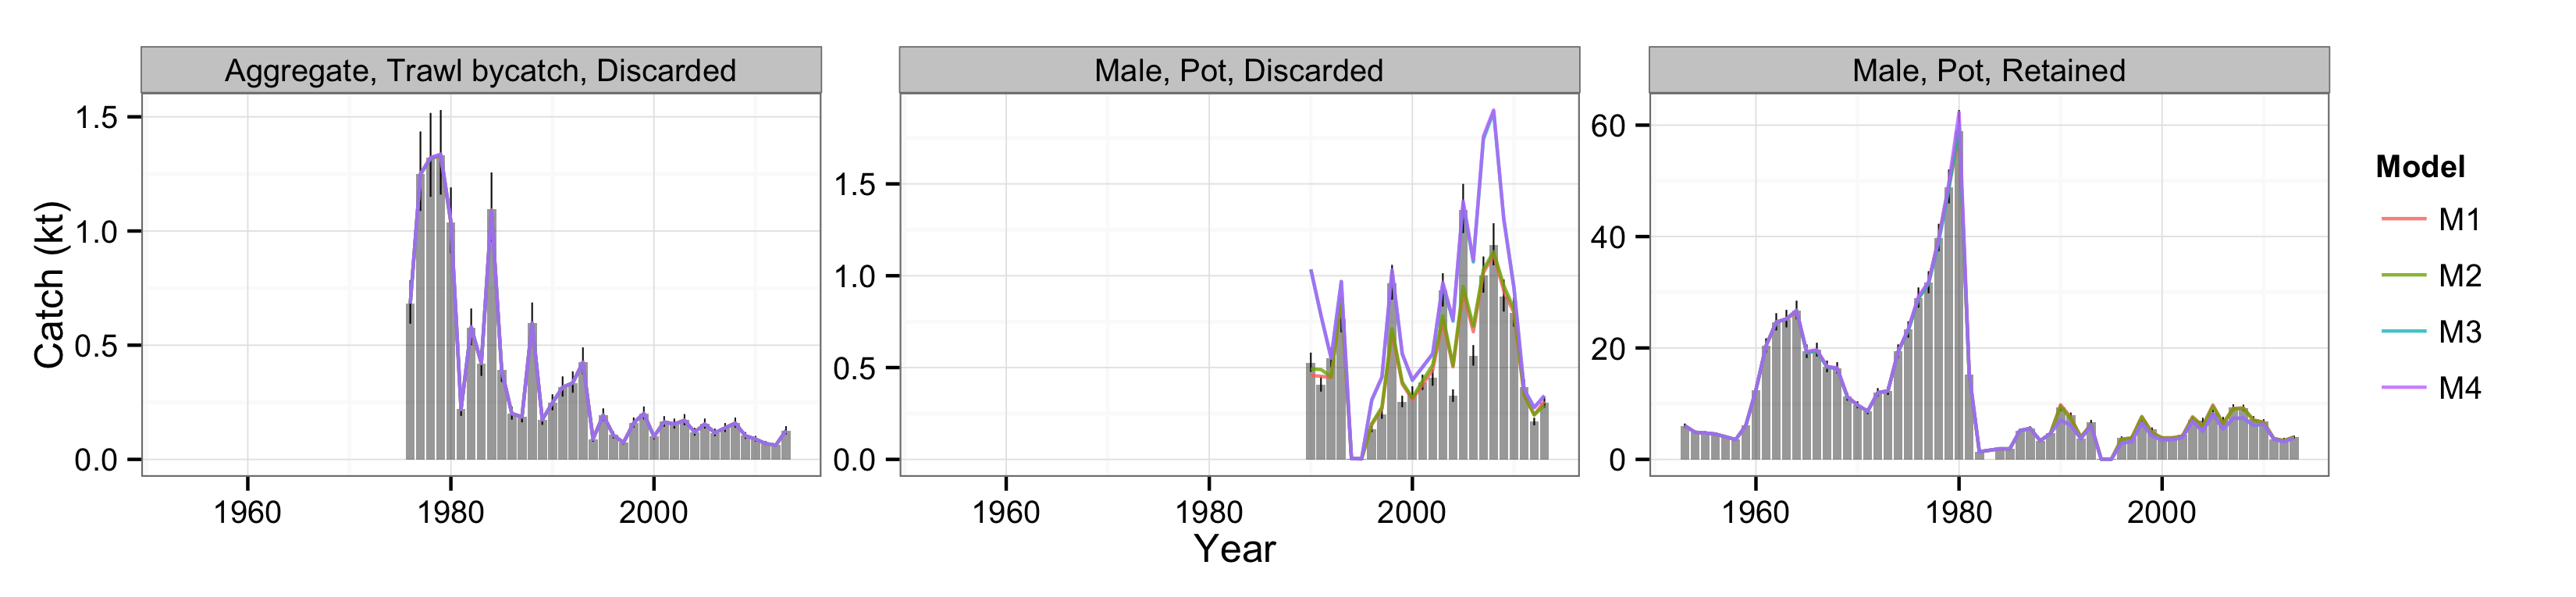
\includegraphics[width=\linewidth]{figCatch.png}\\
          \caption{Observed and predicted catch.}\label{figCatch}
          \end{figure}

          \begin{table}
          \centering
          %\footnotesize
          \caption{SPR-based reference points from each model}
          \begin{tabular}{@{} p{.2\linewidth} c c c c c @{}}
            \toprule
            % Features                                                             & Dim.            & [\%WER] \\
            % Model                                 & F$_{\rm{SPR=35\%}}$  & B$_{\rm{SPR=35\%}}$ \\
            Model & \fspr &  \bspr & \fofl &  OFL & \rspr \\
            \midrule
            \addlinespace
               \textcolor{cM1}{M1} & 0.26  &  22.17 & 0.07  & 0.31  & 5.95 \\
               \textcolor{cM2}{M2} & 0.25  &  33.46 & 0.25  & 3.33  & 7.36 \\
               \textcolor{cM3}{M3} & 0.25  &  25.04 & 0.24  & 1.80  & 5.52 \\
               \textcolor{cM4}{M4} & 0.28  &  28.06 & 0.28  & 2.63  & 7.15 \\
            \bottomrule
          \end{tabular}
          \label{tab:spr_results}
          \end{table} 
        \end{block}
        %%%%%%%%%%%%%%%%%%%%%%%%%%%%%%%%%%%%%%%%%%%%%%%%%%%%%%%%%%%%%%%%%%%%%%%%%%%%%%%

      \end{column}
      %% ------------------------------------------------------------------------------ %%







      %% ------------------------------------------------------------------------------ %%
      %% COLUMN 3
      \begin{column}{.3\linewidth}
        \vspace{3in}
        %%%%%%%%%%%%%%%%%%%%%%%%%%%%%%%%%%%%%%%%%%%%%%%%%%%%%%%%%%%%%%%%%%%%%%%%%%%%%%%
        \begin{block}{\large Results cont.}
          \centering
          
          

          \begin{figure}
          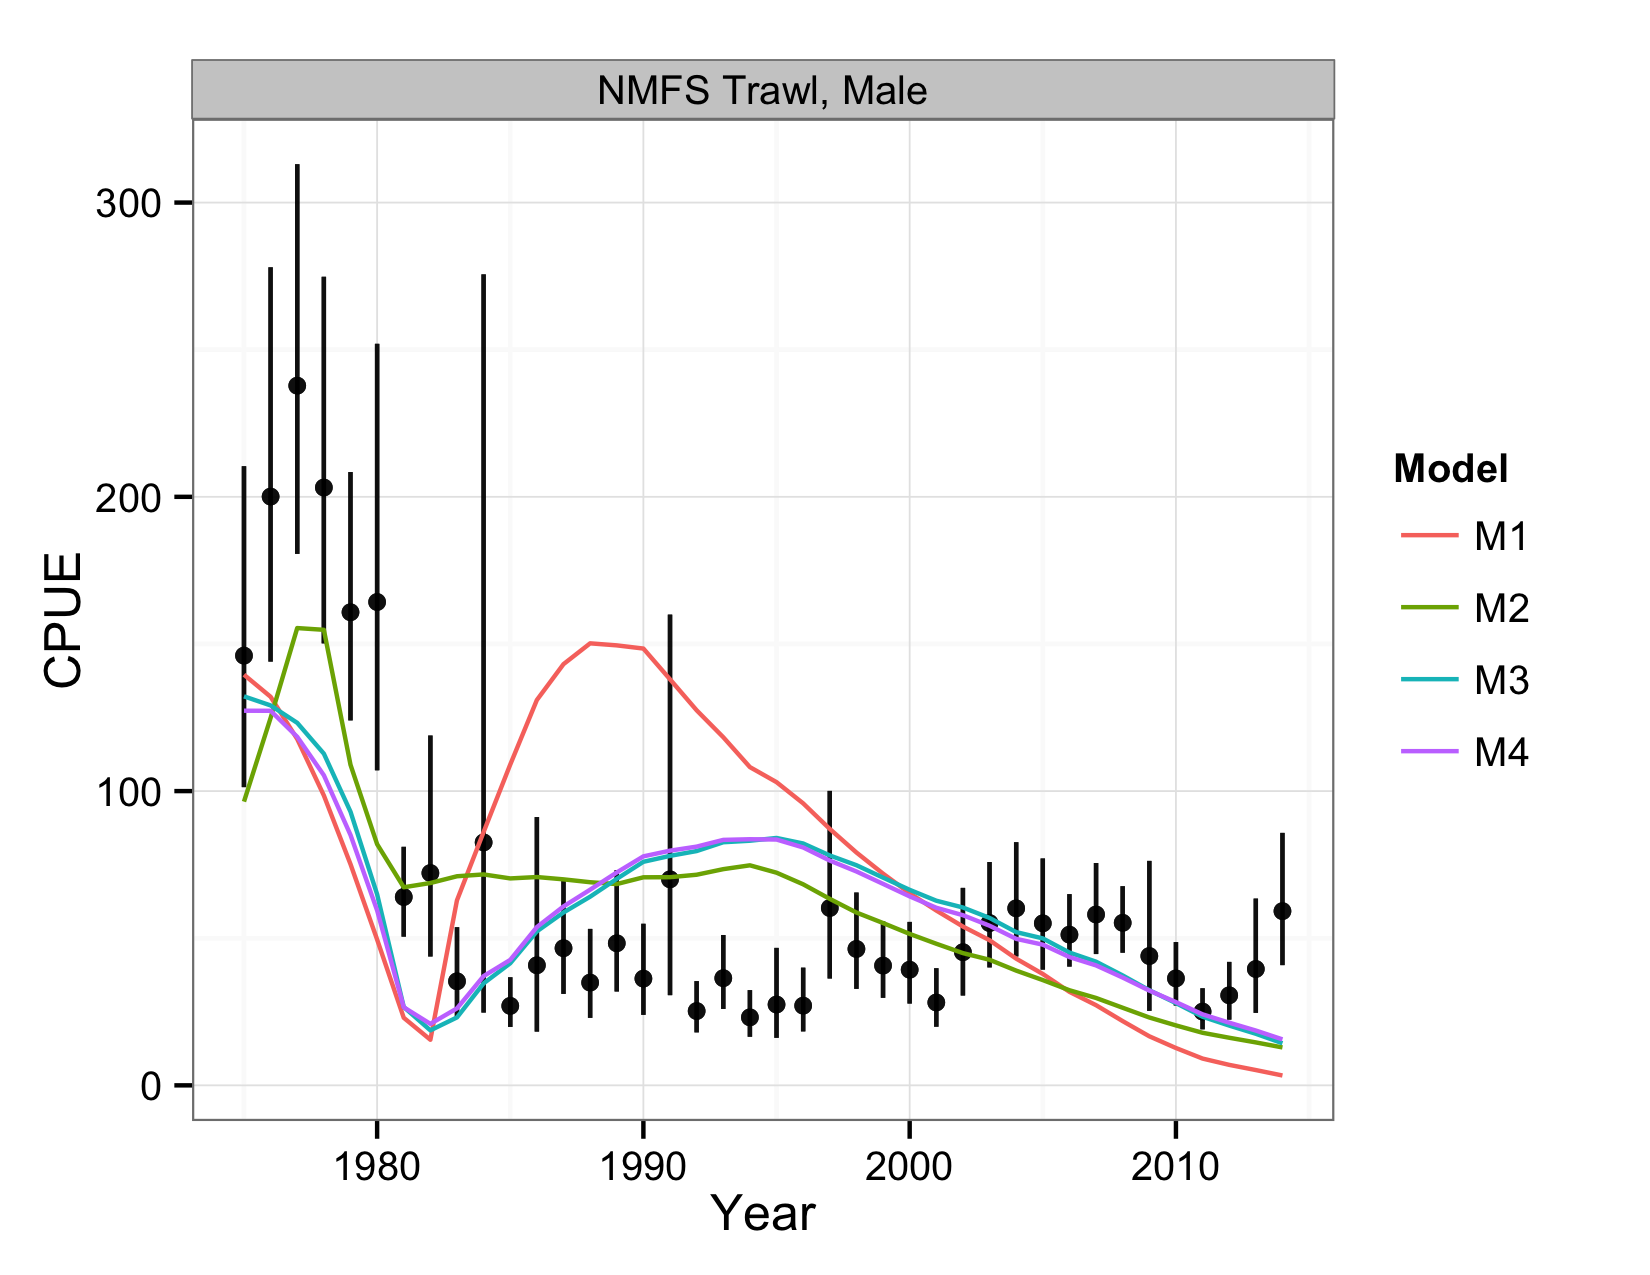
\includegraphics[width=0.5\linewidth]{figCPUE.png}
          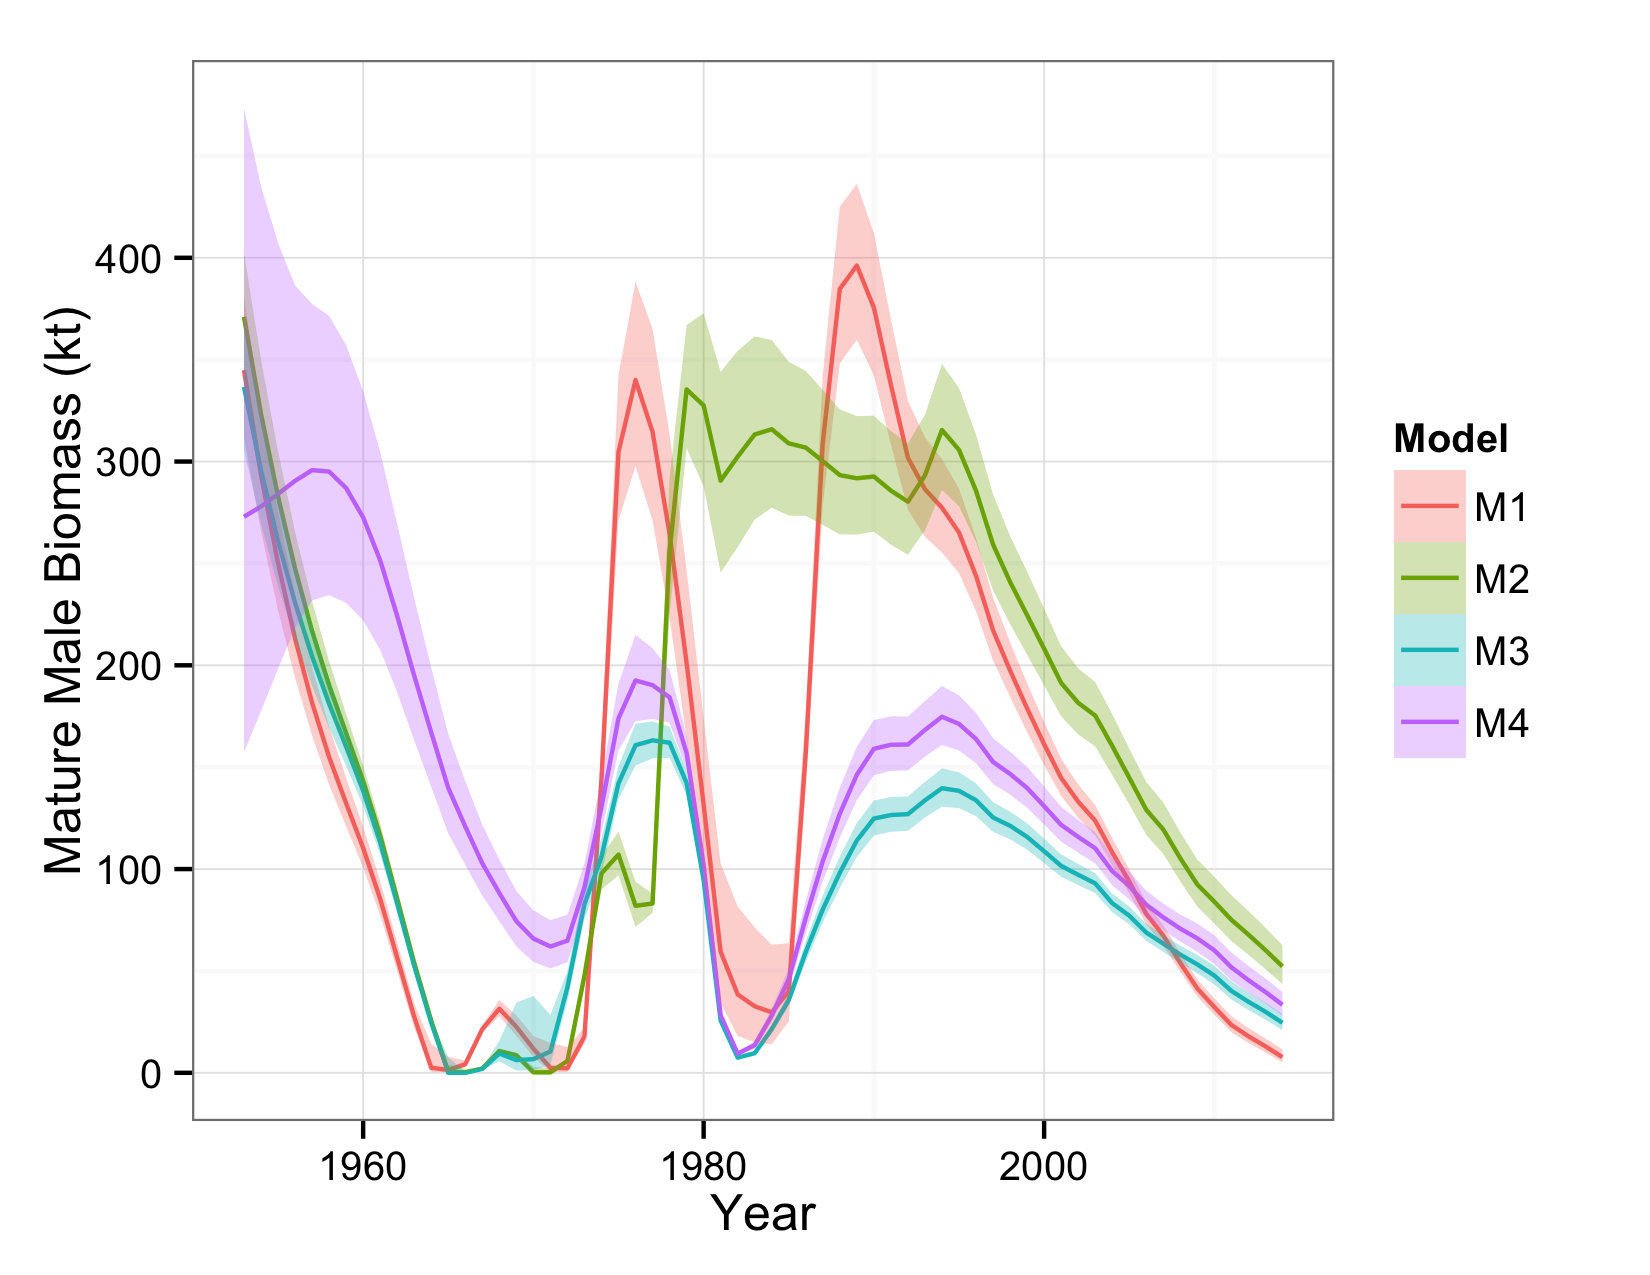
\includegraphics[width=0.5\linewidth]{figMMB.png}\\
          \caption{Fits to relative abundance data (left) and estimates of 
          mature male biomass. Shaded regions approximate 95\% confidence intervals.}
          \label{figCPUE_MMB}
          \end{figure}
          % Observed and predicted CPUE\\

          \begin{figure}
          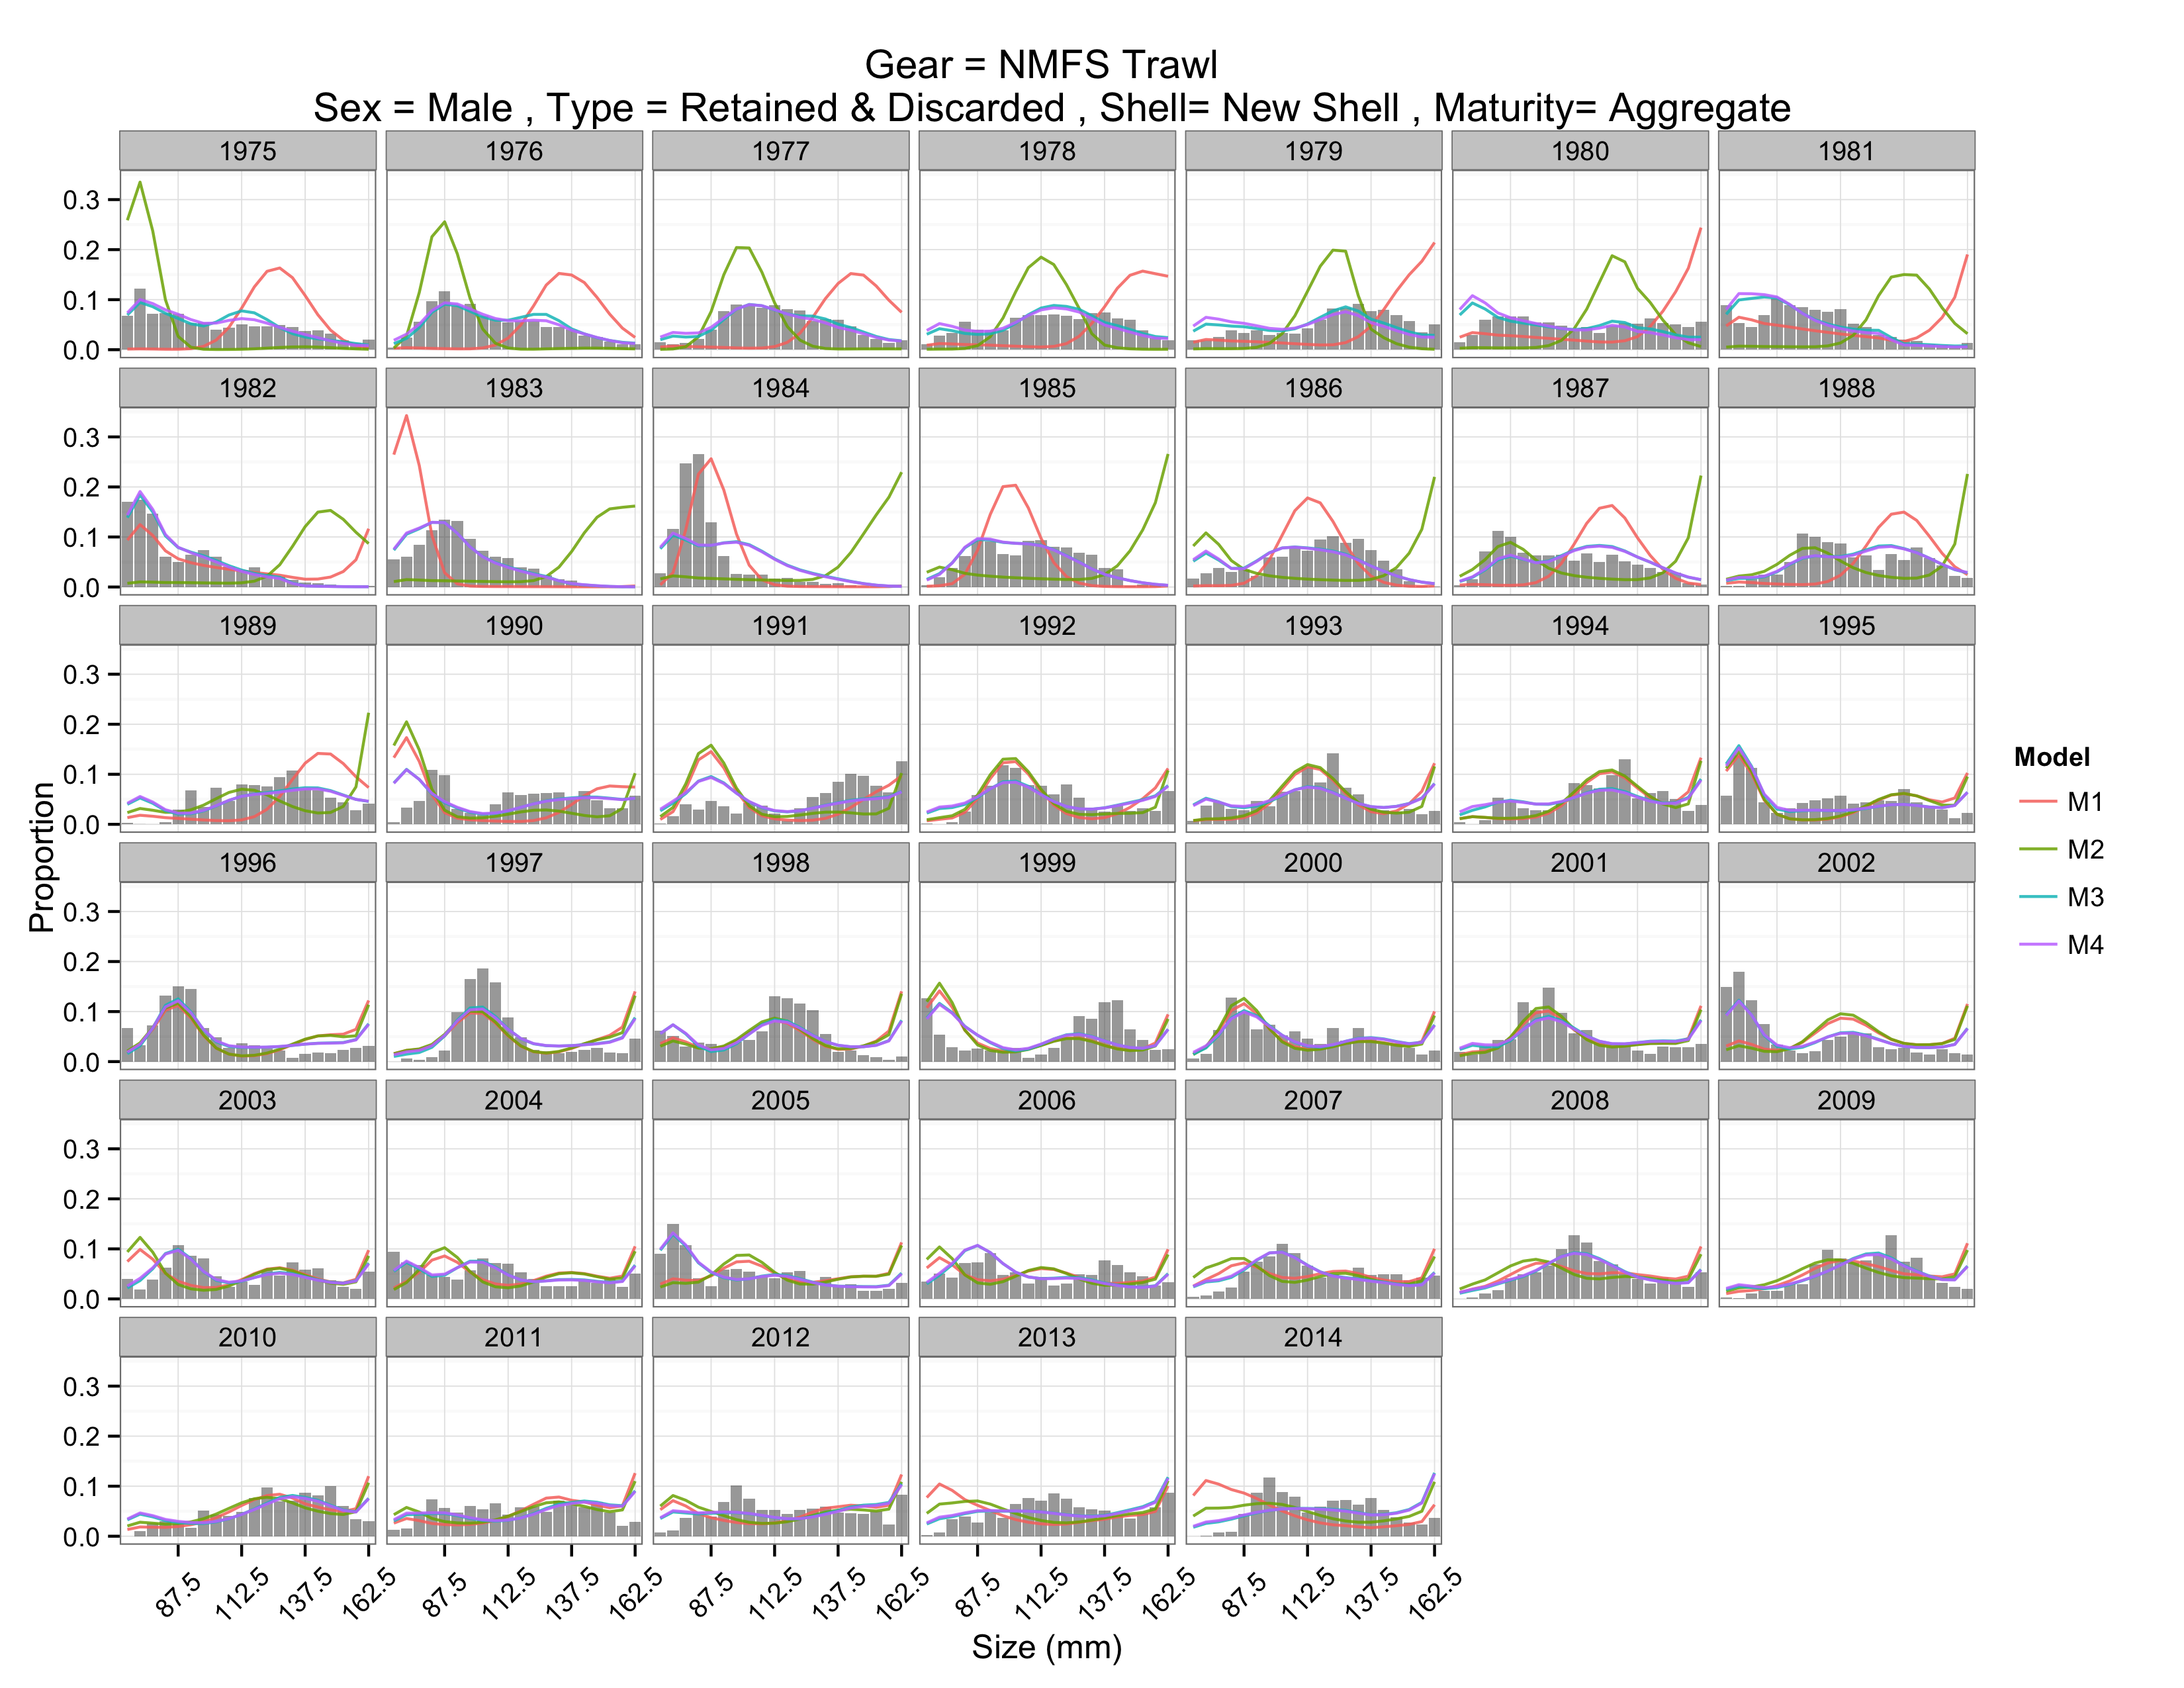
\includegraphics[width=\linewidth]{figSizeComps.png}\\
          \caption{Observed and predicted size composition of newshell crabs in NMFS trawl survey.}
          \label{figSizeComps}
          \end{figure}

        \end{block}
        %%%%%%%%%%%%%%%%%%%%%%%%%%%%%%%%%%%%%%%%%%%%%%%%%%%%%%%%%%%%%%%%%%%%%%%%%%%%%%%
        \vskip1ex
        %%%%%%%%%%%%%%%%%%%%%%%%%%%%%%%%%%%%%%%%%%%%%%%%%%%%%%%%%%%%%%%%%%%%%%%%%%%%%%%
        \begin{block}{\large Discussion}
          \begin{itemize}
            \item Size-structured models contain additional confounding between estimates of recruitment, size-transition, and size-based mortality in contrast to age-structured models.
            \item It is possible to conduct Stock Reduction Analysis (using only catch data) and additional assumptions about natural mortality, growth, and the size-distribution of new recruits.
            \item The generalized size-structured equilibrium model also extends to additional classes such as sex, new and old-shell, immature and mature animals.
          \end{itemize}
        \end{block}
        %%%%%%%%%%%%%%%%%%%%%%%%%%%%%%%%%%%%%%%%%%%%%%%%%%%%%%%%%%%%%%%%%%%%%%%%%%%%%%%
        \vskip1ex
        %%%%%%%%%%%%%%%%%%%%%%%%%%%%%%%%%%%%%%%%%%%%%%%%%%%%%%%%%%%%%%%%%%%%%%%%%%%%%%%
        \begin{block}{\large Acknowledgements}
          Financial support for this project was provided by the Bering Sea Fisheries 
          Research Foundation, NOAA, the North Pacific Fisheries Management Council,
          International Pacific Halibut Commission, and the ADMB Foundation.  We are grateful for the
          contributions from the following people: Jack Turnock, Jie Zheng, Hamachan Hamazaki,
          Athol Whitten, Andr\'e Punt, Darcy Webber and John Levitt.\\[1ex]

          No crabs were eaten during the production of this poster.
          
        \end{block}
        %%%%%%%%%%%%%%%%%%%%%%%%%%%%%%%%%%%%%%%%%%%%%%%%%%%%%%%%%%%%%%%%%%%%%%%%%%%%%%%
        % online api: \url{http://seacode.github.io/gmacs/index.html }
      \end{column}
      %% ------------------------------------------------------------------------------ %%


    % \vfill

      % \begin{column}{.3\linewidth}
      %   \begin{block}{\large Fontsizes}
      %     \centering
      %     {\tiny tiny}\par
      %     {\scriptsize scriptsize}\par
      %     {\footnotesize footnotesize}\par
      %     {\normalsize normalsize}\par
      %     {\large large}\par
      %     {\Large Large}\par
      %     {\LARGE LARGE}\par
      %     {\veryHuge veryHuge}\par
      %     {\VeryHuge VeryHuge}\par
      %     {\VERYHuge VERYHuge}\par
      %   \end{block}
      % \end{column}
      % \vfill

      % \begin{column}{.3\linewidth}
      % %%%%%%%%%%%%%%%%%%%%%%%%%%%%%%%%%%%%%%%%%%%%%%%%%%%%%%%%%%%%%%%%%%%%%%%%%%%%%%%%%%%%%%%%%%%%%%%%%%%%%%%%%%%%

      % \begin{block}{Introduction}
      %   \begin{itemize}
      %   \item automatic sign language recognition system                                    %what
      %   \item \alert{necessary for communication} between deaf and
      %     hearing people
      %   \item \alert{continuous} sign language recognition,
      %     \alert{several} speakers, \alert{vision-based} approach, \alert{no
      %       special hardware}
      %   \item large vocabulary speech recognition (LVSR) system to
      %     obtain a textual representation of the signed
      %     sentences 
      %   \item evaluation of speech recognition techniques on \alert{publicly
      %     available sign language
      %     corpus}
      %   \end{itemize}
      % \end{block}

      % %%%%%%%%%%%%%%%%%%%%%%%%%%%%%%%%%%%%%%%%%%%%%%%%%%%%%%%%%%%%%%%%%%%%%%%%%%%%%%%%%%%%%%%%%%%%%%%%%%%%%%%%%%%%
  
      % \end{column}

      % \begin{column}{.3\linewidth}
      % \end{column}


    \end{columns}

  \end{frame}
\end{document}

